%%%%%%%%%%%%%%%%%%%%%%%%%%%%%%%%%%%%%%%%%%%
%%%%%%%%%%%%%%%%%%%%%%%%%%%%%%%%%%%%%%%%%%%
%%%%%%%%%%%%%%% CHAPTER 15 %%%%%%%%%%%%%%%%


\section{Modelagem: sistemas térmicos}

\frame{
\frametitle{Variáveis}
\begin{block}{Símbolos utilizados}
\begin{itemize}
    \item Os símbolos para as variáveis básicas utilizadas para descrever o comportamento de um sistema térmico são:
    \begin{itemize}
        \item $\theta$, \textbf{temperatura} em kelvins (K)
        \item $q$, \textbf{taxa de fluxo de calor} em metros (J/s = W)
    \end{itemize}
\end{itemize}
\end{block}
}

\frame{
\frametitle{Variáveis}
\begin{block}{Temperatura}
\begin{itemize}
    \item Normalmente, considerando vários pontos de um corpo distribuído, a temperatura difere uma da outra. Para modelagem e análise, assume-se a \textbf{temperatura média do corpo}.
    
    \item Se os desvios de temperatura da média em vários pontos afetam a validade do modelo, então \textbf{o corpo pode ser particionado em segmentos}. Cada um dos segmentos pode ter uma temperatura média diferente associada a ele.
\end{itemize}
\end{block}
}

\frame{
\frametitle{Variáveis}
\begin{block}{Temperatura}
\begin{itemize}
    \item Para a maioria dos sistemas térmicos, existe uma \textbf{condição de equilíbrio} que define a operação nominal. Geralmente, apenas \textbf{desvios das variáveis} de seus valores nominais são de interesse do ponto de vista dinâmico. Neste caso, as \textbf{temperaturas incrementais} são definidas por relações da forma:
    $$\hat{\theta}(t) = \theta(t) - \Bar{\theta}$$
onde $\Bar{\theta}$ é o \textbf{valor nominal}.
\end{itemize}
\end{block}
}

\frame{
\frametitle{Variáveis}
\begin{block}{Temperatura}
\begin{itemize}
    \item A \textbf{temperatura ambiente} ao redor do sistema é constante e é denotada por $\theta_a$. Em alguns problemas, os valores nominais das variáveis de temperatura podem ser iguais a $\theta_a$, caso em que podemos nos referir às temperaturas incrementais como \textbf{temperaturas relativas}.
\end{itemize}
\end{block}
}

\frame{
\frametitle{Variáveis}
\begin{block}{Taxa de fluxo de calor}
\begin{itemize}
    \item Para a maioria dos sistemas térmicos, existe uma \textbf{condição de equilíbrio} que define a operação nominal. Geralmente, apenas \textbf{desvios das variáveis} de seus valores nominais são de interesse do ponto de vista dinâmico. Neste caso, as \textbf{taxas de fluxo de calor incrementais} são definidas por relações da forma:
    $$\hat{q}(t) = q(t) - \Bar{q}$$
onde $\Bar{q}$ é o \textbf{valor nominal}.
\end{itemize}
\end{block}
}

\frame{
\frametitle{Leis dos elementos}
\begin{block}{Quantidade de calor}
\begin{itemize}
    \item Se $q_{in}(t) - q_{out}(t)$ indica a \textbf{taxa líquida de fluxo de calor no corpo em função do tempo}, então o calor líquido fornecido entre o tempo $t_0$ e $t$ é:
    $$\int_{t_0}^{t} [q_{in}(\lambda) - q_{out}(\lambda)] \ d\lambda$$
\end{itemize}
\end{block}
}

\frame{
\frametitle{Leis dos elementos}
\begin{block}{Capacidade térmica}
\begin{itemize}
    \item Existe uma relação algébrica entre a \textbf{temperatura} de um corpo físico e o \textbf{calor armazenado} dentro dele. Desde que não haja mudança de fase e o intervalo de temperaturas não seja excessivo, essa relação pode ser considerada \textbf{linear}.
    \item Assume-se que o calor fornecido durante este intervalo de tempo é igual a uma constante $C$ vezes a \textbf{mudança de temperatura}. Se a temperatura do corpo no tempo de referência $t_0$ é dada por $\theta(t_0)$, então
    $$\int_{t_0}^{t} [q_{in}(\lambda) - q_{out}(\lambda)] \ d\lambda = C[\theta(t) - \theta(t_0)]$$
    ou
    $$\theta(t) = \theta(t_0) + \dfrac{1}{C} \int_{t_0}^{t} [q_{in}(\lambda) - q_{out}(\lambda)] \ d\lambda$$
    onde $C$ é a \textbf{capacidade térmica} (J/K).
\end{itemize}
\end{block}
}

\frame{
\frametitle{Leis dos elementos}
\begin{block}{Capacidade térmica}
\begin{itemize}
    \item Diferenciando
    $$\theta(t) = \theta(t_0) + \dfrac{1}{C} \int_{t_0}^{t} [q_{in}(\lambda) - q_{out}(\lambda)] \ d\lambda$$
    temos
    $$\dot{\theta} = \dfrac{1}{C} [q_{in}(t) - q_{out}(t)]$$
que relaciona a \textbf{taxa de mudança de temperatura} com a taxa instantânea de\textbf{ fluxo de calor líquido} no corpo.
\end{itemize}
\end{block}
}

\frame{
\frametitle{Leis dos elementos}
\begin{block}{Calor específico}
\begin{itemize}
    \item Para um corpo com massa $M$ e \textbf{calor específico} $\sigma$ (J/kg$\cdot$K), a capacidade térmica é dada por:
\end{itemize}
$$C = M \sigma$$
\end{block}
}

\frame{
\frametitle{Leis dos elementos}
\begin{block}{Resistência térmica}
\begin{itemize}
    \item O calor pode fluir entre os pontos por três mecanismos diferentes: \textbf{condução}, \textbf{convecção} e \textbf{radiação}. 
    \item Vamos considerar apenas a \textbf{condução}, onde o calor flui de um corpo para outro, através do meio que os conecta, a uma \textbf{taxa proporcional à diferença de temperatura entre os pontos}. Especificamente, o fluxo de calor por condução de um corpo a uma temperatura $\theta_1$ para um corpo a temperatura $\theta_2$ obedece a seguinte relação:
    $$q(t) = \dfrac{1}{R} [\theta_1(t) - \theta_2(t)]$$
onde $R$ é a \textbf{resistência térmica} (K$\cdot$s/J = K/W).
    \item Para um trajeto de área da secção transversal $A$ e comprimento $d$ composto por material com uma condutividade térmica $\alpha$ (W/m$\cdot$K), a resistência térmica é:
    $$R = \dfrac{d}{A\alpha}$$
\end{itemize}
\end{block}
}

\frame{
\frametitle{Leis dos elementos}
\begin{block}{Fonte térmica}
\begin{itemize}
    \item Existem dois tipos de \textbf{fontes térmicas} ideais. A figura abaixo representa uma fonte que adiciona ou remove calor a uma taxa especificada. 
    \item $q_i(t) > 0$: calor é \textbf{adicionado} ao sistema. 
    \item $q_i(t) < 0$: calor é \textbf{removido} do sistema.
    \item Considera-se a temperatura de um corpo como sendo a \textbf{entrada} do sistema, onde a temperatura é uma função conhecida do tempo, independentemente da taxa que o calor flui entre esse corpo e o resto do sistema.
\end{itemize}
\end{block}
\centerline{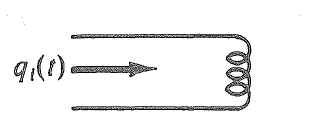
\includegraphics[width=0.3\linewidth]{Figuras/Ch15/fonte.PNG}}
}

\frame{
\frametitle{Exemplo $\#01$ - resistências térmicas em série}
\centerline{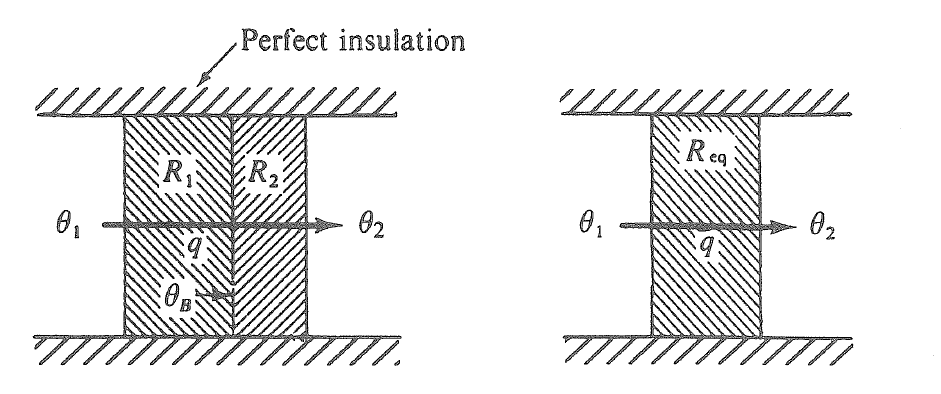
\includegraphics[width=0.7\linewidth]{Figuras/Ch15/fig1.PNG}}
\begin{block}{Problema}
\begin{itemize}
    \item \textbf{Dois corpos} com temperaturas $\theta_1$ e $\theta_2$ separados por duas resistências térmicas $R_1$ e $R_2$.
    \item O \textbf{calor} flui através de cada uma das resistências à uma taxa $q$, mas não pode fluir através do material de \textbf{isolamento} perfeito acima e abaixo das resistências. 
    \item Encontre o valor da \textbf{resistência térmica equivalente} $R_{eq}$ e resolva para a \textbf{temperatura da interface} $\theta_B$.
\end{itemize}
\end{block}
}

\frame{
\frametitle{Exemplo $\#01$ - resistências térmicas em série}
\begin{block}{Solução}
\begin{itemize}
    \item Para o \textbf{primeiro e segundo corpos}, temos, respectivamente:
    \begin{equation*}
    \begin{cases}
    q = \dfrac{1}{R_1} (\theta_1 - \theta_B) \\ \\
    q = \dfrac{1}{R_2} (\theta_B - \theta_2)
    \end{cases}
    \end{equation*}
    \item Para eliminar $\theta_B$, multiplicamos a primeira equação por $R_1$ e a segunda por $R_2$. Somando estas novas equações, chega-se em:
    $$q(R_1 + R_2) = \theta_1 - \theta_2$$
    $$q = \dfrac{1}{R_1 + R_2}(\theta_1 - \theta_2)$$
    \item Logo, $R_{eq} = R_1 + R_2$
\end{itemize}
\end{block}
}

\frame{
\frametitle{Exemplo $\#01$ - resistências térmicas em série}
\begin{block}{Solução}
\begin{itemize}
    \item Para o \textbf{primeiro e segundo corpos}, temos, respectivamente:
    \begin{equation*}
    \begin{cases}
    q = \dfrac{1}{R_1} (\theta_1 - \theta_B) \\ \\
    q = \dfrac{1}{R_2} (\theta_B - \theta_2)
    \end{cases}
    \end{equation*}
    \item Para calcular $\theta_B$, subtraímos as duas equações originais. Logo,
    $$\dfrac{1}{R_1}\theta_1 - \dfrac{1}{R_1}\theta_B - \dfrac{1}{R_2}\theta_B + \dfrac{1}{R_2}\theta_2 = 0 $$
    $$\theta_B \left(\dfrac{1}{R_1} + \dfrac{1}{R_2}\right) = \dfrac{1}{R_1}\theta_1 + \dfrac{1}{R_2}\theta_2$$
    $$\theta_B(R_1 + R_2) = R_2\theta_1 + R_1\theta_2 \implies \theta_B = \dfrac{R_2\theta_1 + R_1\theta_2}{R_1 + R_2}$$
\end{itemize}
\end{block}
}

\frame{
\frametitle{Exemplo $\#02$ - resistências térmicas em paralelo}
\centerline{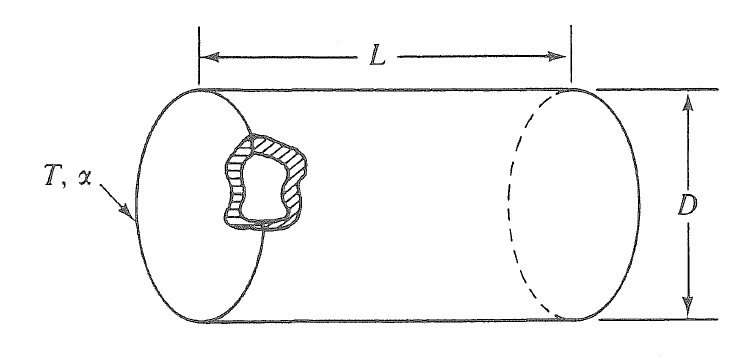
\includegraphics[width=0.6\linewidth]{Figuras/Ch15/fig2.PNG}}
\begin{block}{Problema}
\begin{itemize}
    \item \textbf{Recipiente cilíndrico oco} cujas paredes têm espessura $T$ e um material cuja condutividade térmica é $\alpha$.
    \item Calcule as \textbf{resistências térmicas} da lateral do cilindro ($R_c$) e de cada extremidade ($R_e$).
    \item Após, encontre a \textbf{resistência equivalente} de todo o vaso em termos de $R_c$ e $R_e$.
\end{itemize}
\end{block}
}

\frame{
\frametitle{Exemplo $\#02$ - resistências térmicas em paralelo}
\begin{block}{Solução}
\begin{itemize}
    \item Para a \textbf{lateral do cilindro}, temos:
    $$R_c = \dfrac{T}{\pi D L \alpha} \ \therefore \ q_c = \dfrac{\Delta \theta}{R_c}$$
    \item Para a \textbf{extremidade do cilindro}, temos:
    $$R_e = \dfrac{T}{\dfrac{\pi D^2}{4}\alpha} = \dfrac{4T}{\pi D^2 \alpha} \ \therefore \ q_e = \dfrac{\Delta \theta}{R_e}$$
    \item A taxa \textbf{total} de fluxo de calor é:
    $$q_T = 2q_e + q_c = \left(\dfrac{2}{R_e} + \dfrac{1}{R_c}\right) \Delta \theta = \dfrac{\Delta \theta}{R_{eq}}$$
    \item Logo, $\dfrac{1}{R_{eq}} = \dfrac{2}{R_e} + \dfrac{1}{R_c} \implies R_{eq} = \dfrac{R_c R_e}{2R_c + R_e}$
\end{itemize}
\end{block}
}

\frame{
\frametitle{Exemplo $\#03$ - sistema térmico com uma capacitância}
\centerline{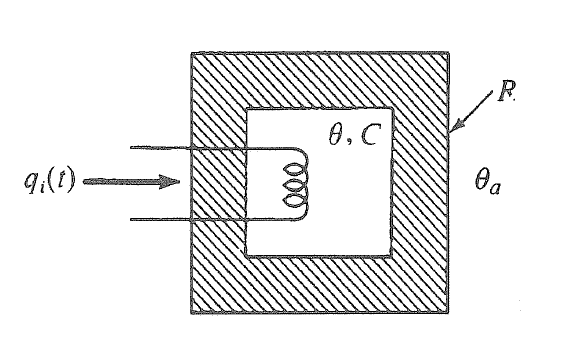
\includegraphics[width=0.4\linewidth]{Figuras/Ch15/fig3.PNG}}
\vspace{-0.3cm}
\begin{block}{Problema}
\begin{itemize}
    \item \textbf{Capacitância térmica} $C$ envolvida por um isolamento que tem uma \textbf{resistência térmica} equivalente $R$.
    \item A \textbf{temperatura} dentro da capacitância é $\theta$, uniforme. A temperatura ambiente ao redor do exterior do isolamento é $\theta_a$, constante.
    \item \textbf{Calor é adicionado} ao interior do sistema a uma taxa $q_i(t)$.
    \item Os \textbf{valores nominais} de $q_i(t)$ e $\theta$ são denotados por $\Bar{q_i}$ e $\Bar{\theta}$.
    \item Encontre o \textbf{modelo do sistema} em termos de $\theta$, $q_i(t)$ e $\theta_a$. Obtenha também o modelo em termos de variáveis incrementais e determine a função de transferência do sistema.
\end{itemize}
\end{block}
}

\frame{
\frametitle{Exemplo $\#03$ - sistema térmico com uma capacitância}
\begin{block}{Solução}
\begin{itemize}
    \item Considerando $q_{in}(t) = q_i(t)$ e $q_{out}(t) = \dfrac{1}{R}(\theta - \theta_a)$, temos:
    $$\dot{\theta} = \dfrac{1}{C} [q_{in}(t) - q_{out}(t)] = \dfrac{1}{C} \Big[q_{i}(t) - \dfrac{1}{R}(\theta - \theta_a)\Big]$$
    \item Com isso, o \textbf{modelo do sistema} em termos de $\theta$, $q_i(t)$ e $\theta_a$ é dado por:
    $$\dot{\theta} + \dfrac{1}{RC}\theta = \dfrac{1}{C}q_i(t) + \dfrac{1}{RC}\theta_a$$
    \item No \textbf{ponto de operação}, temos:
    $$\dfrac{1}{RC}\Bar{\theta} = \dfrac{1}{C}\Bar{q_i} + \dfrac{1}{RC}\theta_a \implies \Bar{\theta} = \theta_a + R\Bar{q_i}$$
\end{itemize}
\end{block}
}

\frame{
\frametitle{Exemplo $\#03$ - sistema térmico com uma capacitância}
\begin{block}{Solução}
\begin{itemize}
    \item Em termos de variáveis incrementais, temos:
    $$\hat{\theta} = \theta - \Bar{\theta}$$
    $$\hat{q_i}(t) = q_i(t) - \Bar{q_i}$$
    \item Substituindo em 
    $$\dot{\theta} + \dfrac{1}{RC}\theta = \dfrac{1}{C}q_i(t) + \dfrac{1}{RC}\theta_a$$
    vem
    $$\dot{\hat{\theta}} + \dot{\Bar{\theta}} + \dfrac{1}{RC}\hat{\theta} + \dfrac{1}{RC} \Bar{\theta} = \dfrac{1}{C}\hat{q_i}(t) + \dfrac{1}{C}\Bar{q_i} + \dfrac{1}{RC}\theta_a$$
\end{itemize}
\end{block}
}

\frame{
\frametitle{Exemplo $\#03$ - sistema térmico com uma capacitância}
\begin{block}{Solução}
\begin{itemize}
    \item Sabendo que $\dot{\Bar{\theta}} = 0$ e lembrando que 
    $$\dfrac{1}{RC}\Bar{\theta} = \dfrac{1}{C}\Bar{q_i} + \dfrac{1}{RC}\theta_a$$
    vem
    $$\dot{\hat{\theta}} + \dfrac{1}{RC}\hat{\theta} + \dfrac{1}{C}\Bar{q_i} + \dfrac{1}{RC}\theta_a = \dfrac{1}{C}\hat{q_i}(t) + \dfrac{1}{C}\Bar{q_i} + \dfrac{1}{RC}\theta_a$$
    $$\dot{\hat{\theta}} + \dfrac{1}{RC}\hat{\theta} = \dfrac{1}{C}\hat{q_i}(t)$$
    \vspace{0.1cm}
    \item A \textbf{função de transferência} é, portanto:
    $$H(s) = \dfrac{\hat{\Theta}(s)}{\hat{Q}(s)}= \dfrac{\dfrac{1}{C}}{s + \dfrac{1}{RC}}$$
\end{itemize}
\end{block}
}

\frame{
\frametitle{Exemplo $\#04$ - sistema térmico com duas capacitâncias}
\centerline{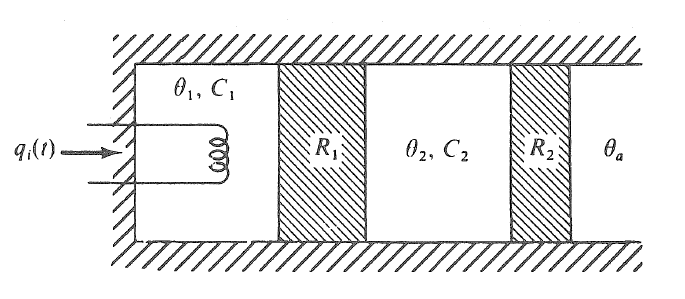
\includegraphics[width=0.6\linewidth]{Figuras/Ch15/fig4.PNG}}
\begin{block}{Problema}
\begin{itemize}
    \item O \textbf{calor} é fornecido, por meio de um radiador, à capacitância esquerda à uma taxa $q_i(t)$.
    \item O calor é perdido na extremidade direita do ambiente, que está a uma temperatura constante $\theta_a$.
    \item O invólucro é considerado \textbf{perfeitamente isolado}, com exceção das \textbf{resistências térmicas} $R_1$ e $R_2$. 
    \item Encontre a \textbf{função de transferência} relacionando as \textbf{variáveis incrementais} $\hat{q}_i(t)$ e $\hat{\theta}_2$.
\end{itemize}
\end{block}
}

\frame{
\frametitle{Exemplo $\#04$ - sistema térmico com duas capacitâncias}
\begin{block}{Solução}
\begin{itemize}
    \item As EDOs que descrevem este sistema são:
    $$\dot{\theta}_1 = \dfrac{1}{C_1} \Big[q_{i}(t) - \dfrac{1}{R_1}(\theta_1 - \theta_2)\Big]$$
    $$\dot{\theta}_2 = \dfrac{1}{C_2} \Big[ \dfrac{1}{R_1}(\theta_1 - \theta_2) - \dfrac{1}{R_2}(\theta_2 - \theta_a)\Big]$$
    \item No \textbf{ponto de operação}, temos:
    $$0 = \dfrac{1}{C_1} \Big[\Bar{q}_i - \dfrac{1}{R_1}(\Bar{\theta}_1 - \Bar{\theta}_2)\Big] \implies \Bar{q}_i - \dfrac{1}{R_1}(\Bar{\theta}_1 - \Bar{\theta}_2) = 0$$
    $$0 = \dfrac{1}{C_2} \Big[ \dfrac{1}{R_1}(\Bar{\theta}_1 - \Bar{\theta}_2) - \dfrac{1}{R_2}(\Bar{\theta}_2 - \theta_a)\Big] \implies \dfrac{1}{R_1}(\Bar{\theta}_1 - \Bar{\theta}_2) - \dfrac{1}{R_2}(\Bar{\theta}_2 - \theta_a) = 0$$
    \item Deste modo,
    $$\Bar{\theta}_1 - \Bar{\theta}_2 = R_1\Bar{q}_i$$
    $$\Bar{\theta}_2 - \theta_a = R_2\Bar{q}_i$$
\end{itemize}
\end{block}
}

\frame{
\frametitle{Exemplo $\#04$ - sistema térmico com duas capacitâncias}
\begin{block}{Solução}
\begin{itemize}
    \item Em termos de variáveis incrementais, temos:
    $$\hat{\theta}_1 = \theta_1 - \Bar{\theta}_1$$
    $$\hat{\theta}_2 = \theta_2 - \Bar{\theta}_2$$
    $$\hat{q}_i(t) = q_i(t) - \Bar{q}_i$$
\end{itemize}
\end{block}
}

\frame{
\frametitle{Exemplo $\#04$ - sistema térmico com duas capacitâncias}
\begin{block}{Solução}
\begin{itemize}
    \item Para a primeira capacitância, temos:
    $$\dot{\hat{\theta}}_1 + \dot{\Bar{\theta}}_1 = \dfrac{1}{C_1}\hat{q}_i(t) + \dfrac{1}{C_1}\Bar{q}_i - \dfrac{1}{C_1R_1}\hat{\theta}_1 - \dfrac{1}{C_1R_1}\Bar{\theta}_1 + \dfrac{1}{C_1R_1}\hat{\theta}_2 + \dfrac{1}{C_1R_1}\Bar{\theta}_2$$
    \item Sabendo que $\dot{\Bar{\theta}}_1 = 0$ e lembrando que 
    $$\Bar{\theta}_1 - \Bar{\theta}_2 = R_1\Bar{q}_i$$
    vem
    $$\dot{\hat{\theta}}_1 + \dfrac{1}{C_1R_1}\hat{\theta}_1 = \dfrac{1}{C_1}\hat{q}_i(t) + \dfrac{1}{C_1}\Bar{q}_i - \dfrac{1}{C_1R_1}(\Bar{\theta}_1 - \Bar{\theta}_2) + \dfrac{1}{C_1R_1}\hat{\theta}_2$$
    $$\dot{\hat{\theta}}_1 + \dfrac{1}{C_1R_1}\hat{\theta}_1 = \dfrac{1}{C_1}\hat{q}_i(t) + \dfrac{1}{C_1R_1}\hat{\theta}_2$$
\end{itemize}
\end{block}
}

\frame{
\frametitle{Exemplo $\#04$ - sistema térmico com duas capacitâncias}
\begin{block}{Solução}
\begin{itemize}
    \item Para a segunda capacitância, temos:
    \begin{equation*}
    \begin{split}
    \dot{\hat{\theta}}_2 + \dot{\Bar{\theta}}_2 =  \dfrac{1}{C_2R_1}\hat{\theta}_1 + \dfrac{1}{C_2R_1}\Bar{\theta}_1 - \dfrac{1}{C_2R_1}\hat{\theta}_2 - \\
    - \dfrac{1}{C_2R_1}\Bar{\theta}_2 - \dfrac{1}{C_2R_2}\hat{\theta}_2 - \dfrac{1}{C_2R_2}\Bar{\theta}_2 + \dfrac{1}{C_2R_2}\theta_a
    \end{split}
    \end{equation*}
    \item Sabendo que $\dot{\Bar{\theta}}_2 = 0$ e lembrando que 
    $$\Bar{\theta}_2 - \theta_a = R_2\Bar{q}_i \ \text{e} \ \Bar{\theta}_1 - \Bar{\theta}_2 = R_1\Bar{q}_i$$
    vem
    $$\dot{\hat{\theta}}_2 + \left(\dfrac{1}{C_2R_1} + \dfrac{1}{C_2R_2}\right)\hat{\theta}_2 = \dfrac{1}{C_2R_1}\hat{\theta}_1 + \dfrac{1}{C_2R_1}(\Bar{\theta}_1 - \Bar{\theta}_2) - \dfrac{1}{C_2R_2}( \Bar{\theta}_2 - \theta_a)$$
    $$\dot{\hat{\theta}}_2 + \left(\dfrac{1}{C_2R_1} + \dfrac{1}{C_2R_2}\right)\hat{\theta}_2 = \dfrac{1}{C_2R_1}\hat{\theta}_1$$
\end{itemize}
\end{block}
}

\frame{
\frametitle{Exemplo $\#04$ - sistema térmico com duas capacitâncias}
\begin{block}{Solução}
\begin{itemize}
    \item Isolando $\hat{\theta}_1$ na última equação, têm-se que
    $$\hat{\theta}_1 = C_2R_1\dot{\hat{\theta}}_2 + \left(1 + \dfrac{R_1}{R_2}\right)\hat{\theta}_2$$
    \item Substituindo esta na primeira equação,
    $$\dot{\hat{\theta}}_1 + \dfrac{1}{C_1R_1}\hat{\theta}_1 = \dfrac{1}{C_1}\hat{q}_i(t) + \dfrac{1}{C_1R_1}\hat{\theta}_2$$
    vem
    \begin{equation*}
    \begin{split}
    C_2R_1\ddot{\hat{\theta}}_2 + \left(1 + \dfrac{R_1}{R_2}\right)\dot{\hat{\theta}}_2 + \dfrac{1}{C_1R_1}\Big[C_2R_1\dot{\hat{\theta}}_2 + \left(1 + \dfrac{R_1}{R_2}\right)\hat{\theta}_2\Big] = \\
    \dfrac{1}{C_1R_1}\hat{\theta}_2 + \dfrac{1}{C_1}\hat{q}_i(t) 
    \end{split}
    \end{equation*}
\end{itemize}
\end{block}
}

\frame{
\frametitle{Exemplo $\#04$ - sistema térmico com duas capacitâncias}
\begin{block}{Solução}
\begin{itemize}
    \item Rearrumando, chega-se em
    $$C_2R_1\ddot{\hat{\theta}}_2 + \left(1 + \dfrac{R_1}{R_2} + \dfrac{C_2}{C_1}\right)\dot{\hat{\theta}}_2 + \left(\dfrac{1}{C_1R_1} + \dfrac{1}{C_1R_2} - \dfrac{1}{C_1R_1}\right)\hat{\theta}_2 = \dfrac{1}{C_1}\hat{q}_i(t)$$
    $$\ddot{\hat{\theta}}_2 + \left(\dfrac{1}{C_2R_1} + \dfrac{1}{C_2R_2} + \dfrac{1}{C_1R_1}\right)\dot{\hat{\theta}}_2 + \dfrac{1}{C_1C_2R_1R_2}\hat{\theta}_2 = \dfrac{1}{C_1C_2R_1}\hat{q}_i(t)$$
    \vspace{0.1cm}
    \item A \textbf{função de transferência} é, portanto:
    $$H(s) = \dfrac{\hat{\Theta}_2(s)}{\hat{Q}_i(s)}= \dfrac{\dfrac{1}{C_1C_2R_1}}{s^2 + \left(\dfrac{1}{C_2R_1} + \dfrac{1}{C_2R_2} + \dfrac{1}{C_1R_1}\right)s + \dfrac{1}{C_1C_2R_1R_2}}$$
\end{itemize}
\end{block}
}

\frame{
\frametitle{Exemplo $\#05$ - sistema térmico aproximado por uma capacitância}
\centerline{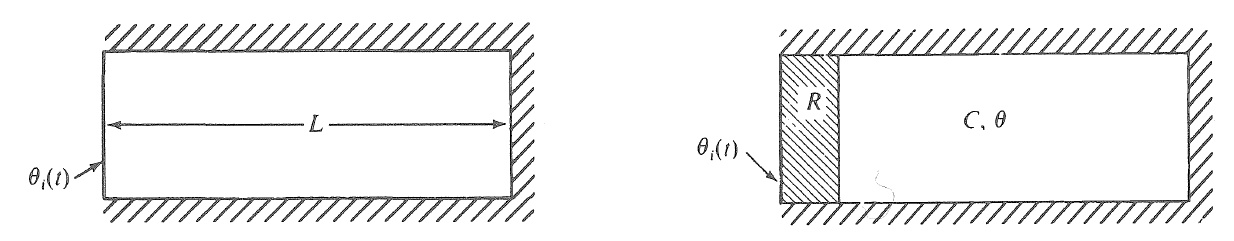
\includegraphics[width=1\linewidth]{Figuras/Ch15/fig5.PNG}}
\begin{block}{Problema}
\begin{itemize}
    \item Considere uma \textbf{barra} de comprimento $L$ e área $A$ que é perfeitamente isolada em todos as partes, exceto na extremidade esquerda.
    \item A \textbf{temperatura} na extremidade esquerda da barra é $\theta_i(t)$, uma função conhecida do tempo que é a \textbf{entrada do sistema}.
    \item O interior da barra está inicialmente na temperatura ambiente $\theta_a$. O calor específico é $\sigma$, sua densidade é $\rho$ e sua condutividade térmica é $\alpha$.
    \item Embora o sistema seja \textbf{distribuído}, desenvolva um modelo \textbf{aproximado} consistindo de uma capacitância e uma resistência térmica e, em seguida, encontre a resposta ao \textbf{degrau unitário}.
\end{itemize}
\end{block}
}

\frame{
\frametitle{Exemplo $\#05$ - sistema térmico aproximado por uma capacitância}
\begin{block}{Solução}
\begin{itemize}
    \item Assume-se todos os pontos internos com uma mesma temperatura $\theta$, com exceção da extremidade esquerda cuja temperatura é $\theta_i(t)$.
    $$\rho = \dfrac{M}{V} \implies M = \rho \cdot V = \rho \cdot AL$$
    Com isso,
    $$C = \sigma M = \sigma \rho AL$$
    \item Considerando $q_{in}(t) = \dfrac{1}{R}[\theta_i(t) - \theta]$ e $q_{out} = 0$ (isolamento perfeito):
    $$\dot{\theta} = \dfrac{1}{C} [q_{in}(t) - q_{out}(t)] = \dfrac{1}{RC} \Big[\theta_i(t) - \theta\Big]$$
    \item Com isso, o \textbf{modelo do sistema} é dado por:
    $$\dot{\theta} + \dfrac{1}{RC}\theta = \dfrac{1}{RC}\theta_i(t)$$
\end{itemize}
\end{block}
}

\frame{
\frametitle{Exemplo $\#05$ - sistema térmico aproximado por uma capacitância}
\begin{block}{Solução}
\begin{itemize}
    \item Se a temperatura $\theta_i(t)$ é a soma da temperatura ambiente constante $\theta_a$ e uma função de degrau da altura B, podemos escrever
    $$\theta_i(t) = \theta_a + Bu(t)$$
    \item Neste exemplo, é conveniente definir os valores nominais das temperaturas como sendo a temperatura ambiente $\theta_a$ e escrever as variáveis incrementais como sendo as temperaturas relativas a $\theta_a$. Deste modo,
    $$\hat{\theta}_i(t) = \theta_i(t) - \theta_a = Bu(t)$$
    $$\hat{\theta} = \theta - \theta_a$$
\end{itemize}
\end{block}
}

\frame{
\frametitle{Exemplo $\#05$ - sistema térmico aproximado por uma capacitância}
\begin{block}{Solução}
\begin{itemize}
    \item Com isso,
    $$\dot{\hat{\theta}} + \dfrac{1}{RC}(\hat{\theta} + \theta_a) = \dfrac{1}{RC}[\theta_a + Bu(t)] \implies \dot{\hat{\theta}} + \dfrac{1}{RC}\hat{\theta} = \dfrac{B}{RC}u(t)$$
    \item A \textbf{função de transferência} é, portanto:
    $$H(s) = \dfrac{\hat{\Theta}(s)}{U(s)} = \dfrac{B\dfrac{1}{RC}}{s+\dfrac{1}{RC}}$$
    \item Para $U(s) = 1/s$, temos:
    $$\hat{\theta} = B\big(1 - \text{e}^{-t/RC}\big)$$
    onde $\tau = RC = \dfrac{\sigma \rho L^2}{\alpha}$ é a constante de tempo.
\end{itemize}
\end{block}
}

\frame{
\frametitle{Exercícios}
\begin{block}{}
01. Determine as EDOs, em termos de variáveis incrementais, da barra isolada de um sistema térmico aproximado por duas capacitâncias, vista na figura abaixo.
\end{block}
\centerline{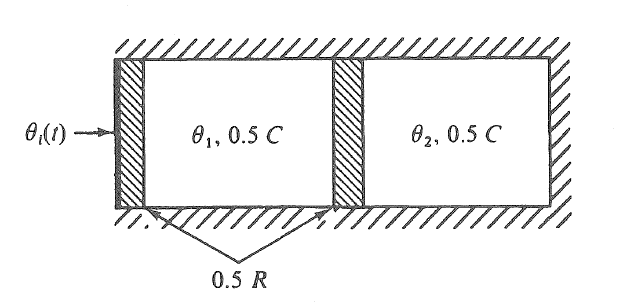
\includegraphics[width=0.6\linewidth]{Figuras/Ch15/fig6.PNG}}
}

\frame{
\frametitle{Referências e exercícios complementares}
\begin{itemize}
\item CLOSE, Charles M.; FREDERICK, Dean K.; NEWELL, Jonathan C. Modeling and Analysis of Dynamic Systems, 3 ed. John Wiley \& Sons, 2003.
\end{itemize}
\centering{\alert{Página 390 - \textbf{Capítulo 11}}} \\
}